\section{Вращательное движение твердого тела}

\introProblems

\begin{ex} %Сив362
Стержень массы $M$ и длины $l$, который может свободно вращаться вокруг неподвижной горизонтальной оси, проходящей через один из его концов, под действием силы тяжести переходит из горизонтального положения в вертикальное (рис. \ref{rodHitMass}). Проходя через вертикальное положение, нижний конец стержня упруго ударяет о малое тело массы $m$, лежащее на гладком горизонтальном столе. Определить скорость тела $m$ после удара.
\begin{ans}
$v = 2M\sqrt{3gl}/(M+3m)$.
\end{ans}
\end{ex}	

\begin{figure}[h]
\centering
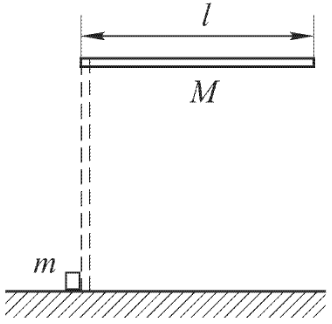
\includegraphics[width=0.35\textwidth]{rodHitMass.png}
\caption{}
\label{rodHitMass}
\end{figure}

\begin{ex} %Сив373
На двух параллельных горизонтальных брусьях лежит сплошной цилиндр радиуса $R$ и массы $m$, на который намотана веревка. К опущенному вниз концу веревки приложена вертикальная сила $F$, равная половине веса цилиндра (рис. \ref{rollingCylinder2}). Найти горизонтальное ускорение цилиндра и минимальное значение коэффициента трения между цилиндром и брусьями, при котором будет происходить качение без скольжения. Ось цилиндра перпендикулярна к брусьям, центр его масс и сила $F$ лежат в вертикальной плоскости, проходящей посередине между брусьями.
\begin{ans}
$a = g/3$, при $\mu \leq 2/9$.
\end{ans}
\end{ex}	

\begin{figure}[h]
\centering
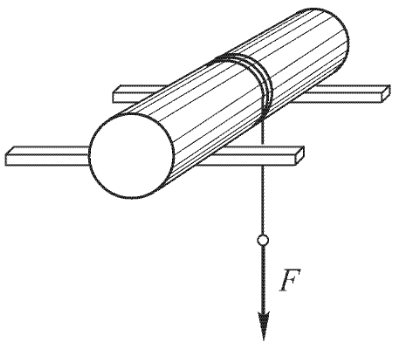
\includegraphics[width=0.4\textwidth]{rollingCylinder2.png}
\caption{}
\label{rollingCylinder2}
\end{figure}

\begin{ex} %Сив393
Сплошной однородный шар радиуса $r$, вращающийся вокруг горизонтального диаметра с угловой скоростью $\omega_0$, ставится на горизонтальную плоскость без сообщения ему поступательного движения. Учитывая трение скольжения, но пренебрегая трением качения, найти линейную скорость $v$ центра шара, когда его движение перейдет в чистое качение. Определить потерю кинетической энергии на трение.
\begin{ans}
$v = 2/7r \omega_0$, $\Delta E = 1/7 mr^2 \omega_0^2$.
\end{ans}
\end{ex}	

\qualProblems

\begin{ex}
Может ли одна сила, приложенная к твердому телу, изменить его поступательное движение и вращательное движение?
\end{ex}	

\begin{ex}
Когда канатоходец идет по канату, он расставляет руки в стороны для того чтобы сохранять равновесие. Объясните этот механизм с точки зрения основного уравнения вращательного движения твердого тела.
\end{ex}	

\simpleProblems

\begin{ex} %Сив366
Вертикальный столб высотой $l$ подпиливается у основания и падает на землю, поворачиваясь вокруг нижнего основания. Определить линейную скорость его верхнего конца в момент удара о землю. Какая точка столба будет в этот момент иметь ту же скорость, какую имело бы тело, падая с той, же высоты, как и данная точка?
\begin{ans}
$v = \sqrt{3gl}$, $x = 2/3l$.
\end{ans}
\end{ex}	

\begin{ex} %Сив369
Гимнаст на перекладине выполняет большой оборот из стойки на руках, т.е. вращается, не сгибаясь, вокруг перекладины под действием собственного веса. Оценить приближенно наибольшую нагрузку $F$ на его руки, пренебрегая трением ладоней о перекладину.
\begin{ans}
Если при оценке человека моделировать однородным стержнем, получим $F = 4mg$.
\end{ans}
\end{ex}	

\begin{ex} %Сив379
К шкиву креста Обербека (рис. \ref{oberbek}) прикреплена нить, к которой подвешен груз массы $M = 1$ кг. Груз опускается с высоты $h = 1$ м до нижнего положения, а затем начинает подниматься вверх. В это время происходит «рывок», т.е. увеличение натяжения нити. Найти натяжение нити $T$ при опускании или поднятии груза, а также оценить приближенно натяжение во время рывка $T_1$. Радиус шкива $r = З$ см. На кресте укреплены четыре груза с массой $m = 250$ г каждый на расстоянии $R = 30$ см от его оси. Моментом инерции самого креста и шкива пренебречь по сравнению с моментом инерции грузов. Растяжение нити во время рывка не учитывать.
\begin{ans}
$T = Mg/(1 + Mr^2/(4mR^2))$, $T_1 = Mg + MhrT/(\pi m R^2)$.
\end{ans}
\end{ex}	

\begin{figure}[h]
\centering
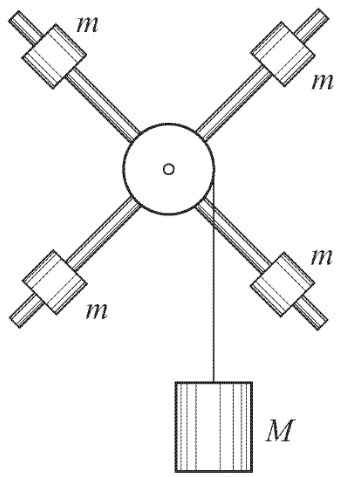
\includegraphics[width=0.3\textwidth]{oberbek.png}
\caption{}
\label{oberbek}
\end{figure}

\complexProblems

\begin{ex} %Сив374
К концу веревки, намотанной на цилиндр привязан груз массы $M$. Веревка переброшена через блок, как показано на рис. \ref{slipCylinder}. Определить ускорение груза $M$. Выяснить условия, при которых качение цилиндра будет происходить со скольжением. Весом веревки и блока, а также силами трения на оси блока можно пренебречь. Считать, что во всех случаях движение цилиндра будет плоскопараллельным.
\begin{ans}
$a = g/(1+3m/8M)$, при отсутствии скольжения $\mu /leq (8+3m/M)^{-1}$; $a = g(1 - \mu m/3M)/(1+m/3M)$, при скольжении $\mu < (8+3m/M)^{-1}$.
\end{ans}
\end{ex}	

\begin{figure}[h]
\centering
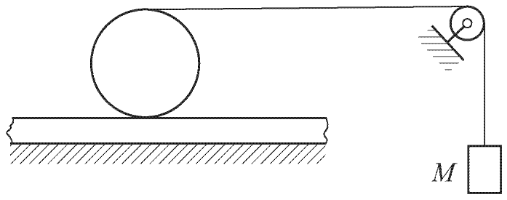
\includegraphics[width=0.5\textwidth]{slipCylinder.png}
\caption{}
\label{slipCylinder}
\end{figure}

\begin{ex} %Сив376
Два катка, связанные штангой $S$, скатываются без скольжения с наклонной плоскости, образующей угол в $30^{\circ}$ с горизонтом (рис. \ref{2rolling}). Катки имеют одинаковые массы $m = 5$ кг и одинаковые радиусы $R = 5$ см, момент инерции первого $I_1 = 80$ кгсм\textsuperscript{2}, второго $I_2 = 40$ кгсм\textsuperscript{2}. Массами рам катков и штанги можно пренебречь. Подсчитать угловое ускорение, с которым катки скатываются без скольжения с наклонной плоскости. Определить силу, передаваемую штангой, если каток с большим моментом инерции движется впереди, и наоборот.
\begin{ans}
$\varepsilon = \frac{2Rg \sin \alpha}{(I_1 + I_2)/m + 2R^2} \approx 66$ c\textsuperscript{-2}.
\end{ans}
\end{ex}	

\begin{figure}[h]
\centering
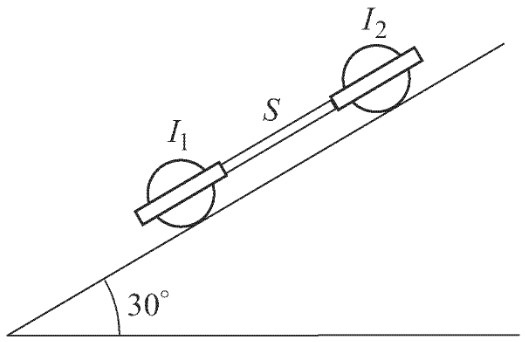
\includegraphics[width=0.5\textwidth]{2rolling.png}
\caption{}
\label{2rolling}
\end{figure}

\begin{ex} %Сив391
Сплошной цилиндр, ось которого горизонтальна, движется без вращения по гладкой горизонтальной плоскости в направлении, перпендикулярном к его оси. В некоторый момент цилиндр достигает границы, где поверхность становится шероховатой и возникает постоянная (не зависящая от скорости) сила трения скольжения, а трение качения отсутствует. Каково будет движение цилиндра после перехода границы? Как распределится кинетическая энергия поступательного движения цилиндра?
\begin{ans}
Движение после перехода границы будет сначала равнозамедленное, а затем с постоянной скоростью; 1/3 энергии превратится в тепло, 2/9 — во вращательную энергию и 4/9 останется в виде энергии поступательного движения.
\end{ans}
\end{ex}	

\begin{ex} %Сив383

\begin{figure}[h]
\centering
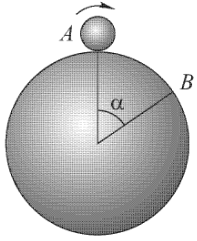
\includegraphics[width=0.25\textwidth]{ballSphere.png}
\caption{}
\label{ballSphere}
\end{figure}

Шарик радиуса $r$ скатывается без начальной скорости и без скольжения по поверхности сферы из самого верхнего положения $A$ (рис. \ref{ballSphere}). Определить положение точки $B$, в которой он оторвется от сферы и начнет свободно двигаться под действием силы тяжести.
\begin{ans}
$\cos \alpha = 10/17$.
\end{ans}
\end{ex}	

\clearpage